\documentclass[a4paper,12pt]{article}
\usepackage[left=1cm,right=1cm,top=3cm,bottom=3cm,a4paper]{geometry}
\usepackage[pdftex]{graphicx}
\usepackage{graphicx}
\usepackage{kotex}
\newcommand{\dbar}{d\hspace*{-0.08em}\bar{}\hspace*{0.1em}}
\usepackage[onehalfspacing]{setspace}
\begin{document}
	\begin{flushleft}
		$<$준-정적 과정(Quasi-static process)- 에너지의 fluctuation으로부터 계가 한 일 구하기$>$ $\rightarrow$ 교과서 3-2번 문제! 이 문제를 풀기전에 다음 주제들을 알면 해답지를 이해하기가 그나마 쉬움 
	\end{flushleft}
\paragraph{}
$\bullet$ 준-정적 과정이란? fluctuation을 주는 주기가 equilibrium으로 돌아가는 시간에 비해 길 때 $\bullet$\\
system의 크기변수가 $x_1,\cdots,x_n$의 값을 가질 때, 유한한 양자 상태 $r$에서 system의 에너지는 다음과 같은 값을 갖는다.
$$E_r=E_r(x_1,\cdots,x_n)$$
크기변수가 각각의 $a$에 대하여 $x_a\rightarrow x_a+dx_a$ 만큼씩 변하면 총 에너지의 변화는 다음과 같다.(total differential)
$$dE_r=\sum_{a=1}^{n}\frac{\partial E_r}{\partial x_a}dx_a$$ 
열역학 제 1법칙
$$dE=\dbar Q-\dbar W$$
에서 $\dbar Q=0$ 이므로, 계가 한 일은 다음과 같다.
$$\dbar W_{r}=-dE_{r}=\sum_{a=1}^{n}\left( -\frac{\partial E_r}{\partial x_a}\right) dx_a=\sum_{a=1}^{n}X_{a,r}dx_a,\quad\mbox{where }X_{a,r}\equiv -\frac{\partial E_r}{\partial x_a}$$
note that 
$$\int F(x)dx=E(x), \quad F(x)=\frac{dE}{dx}$$
위의 note에서 만약 $x_a$가 거리를 나타내는 크기변수라면 $X_{a}$ 는 힘을 나타낸다는 것을 알 수 있다.  계의 크기변수가 quasi-static하게 변하면 일반화한 힘 $X_{a,r}$ 은 언제나 well define 된 평균값을 가진다. 일반화한 힘에 대해서 모든 가능한 양자 상태 $r$에 대한 평균값을 $<X_{a}>$ 로 적는다면, 계가 평균적으로 한 일은 다음과 같다.
$$\dbar W=\sum_{a=1}^{n}<X_{a}>dx_a, \quad \mbox{where }<X_a>\equiv \left\langle -\frac{\partial E_r}{\partial x_a} \right\rangle $$
간단한 예로, 다음의 실린더를 보자. 피스톤이 움직이기 전, 이 실린더는 원래 $V$의 부피를 가지고 있었다. 지금 이 실린더 계는 어떤 양자 상태 $r$에 있고, 넓이 $A$ 인 피스톤에 압력 $p_r$ 을 작용하고 있다.  
\begin{figure}[h]
	\centering
	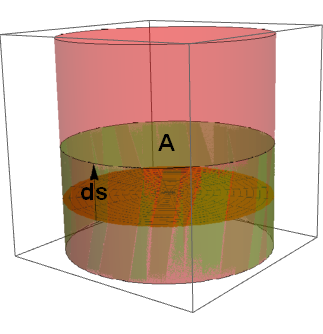
\includegraphics[width=0.2\columnwidth]{cylinder.png}
	\end{figure}
\\계가 피스톤에 작용하는 힘은 $p_r A$이고 실린더 바닥에서 피스톤까지의 거리는 $s$, 즉, 계의 현재 부피는 $V=As$이다. 계가 팽창해서 거리 $s$가 $ds$ 만큼 변하면 계는 이 양자 상태 $r$에 그대로 남아있고,
$$\dbar W_{r}=(p_r A)ds=p_r(Ads)=p_r dV$$ 의 일을 한다. $\dbar W_r=-dE_r$ 에서 $$p_r=-\frac{\partial E_r}{\partial V}$$
앞에서의 논의에 따라 $p_r$ (압력) 은 크기변수 $V$ (부피)에 대응하는 `일반화 된 힘'이다.
\paragraph{}
$\bullet$ 크기변수에 대한 상대밀도의 의존성 $\bullet$\\
한 개 이상의 크기변수가 변할 때 역학적인 상호작용에 대해서 알아보자($\dbar Q=0$). 간단하게 하기 위해 단 하나의 크기변수 $x$ 만 자유롭게 변할 수 있다고 가정하자. 일반적으로 에너지가 $E$ 에서 $E+\delta E$ 사이에 놓여있는 총 상태의 수 $\Omega$ 는 $x$와 $E$에 대한 함수로 나타낼 수 있다. 이렇게 $\longrightarrow \Omega(E,x)$\\
$x$가 $dx$ 만큼 변할 때 특정 양자 상태 $r$ 의 에너지 $E_r(x)$는 다음과 같이 변한다. (어디선가 보았을 것이다.) $$\left( \frac{\partial E_r}{\partial x} \right)dx $$
이제 새로운 상태 수를 정의하자. $x$가 $dx$만큼 변하는 동안 에너지가 $E$보다 작은 상태에서 $E$보다 큰 상태로 넘어간 경우의 총 수를 $\sigma(E,x)$라고 할 것이다.(이 부분은 Reif책 3.8절의 내용임) \\
 이러한 상태들의 수는 단위 에너지당 상태 수 ($\Omega/\delta E$) 에 에너지 범위 ($(\partial E_r/\partial x)dx$) 의 평균을 곱한 값
 $$\sigma(E,x)=\frac{\Omega(E,x)}{\delta E}\left\langle  \frac{\partial E_r}{\partial x}\right\rangle  dx$$ 으로 주어진다. (더 자세한 설명은 Reif책 3.8절 112쪽에 있음) 또는 다음과 같이 쓸 수 있다.
 $$\sigma(E,x)=-\frac{\Omega(E,x)}{\delta E}\langle X \rangle dx$$
 Consider the total number of microstates between $E$ and $E+\delta E$. When the external parameter changes from $x$ to $x+dx$, the number of states in this energy range changes by $(\partial\Omega/\partial x)dx$. This change is due to the difference between the number of states which `enter' the range bacause their energy is changed from a value less than $E$ to one greater than $E$ and the number which `leave' because their energt is changed from a value less than $E+\delta E$ to one greater than $E+\delta E$. In symbols,
 $$\frac{\partial \Omega(E,x)}{\partial x}dx=\sigma(E)-\sigma(E+\delta E)\simeq-\frac{\partial \sigma}{\partial E}\delta E$$
 $$=(-\frac{\partial}{\partial E})(-\frac{\Omega(E,x)}{\delta E} \langle X \rangle dx)\delta E$$
 따라서, 
 $$\frac{\partial \Omega}{\partial x}=\frac{\partial(\Omega \langle X \rangle )}{\partial E}$$
 $$=\langle X \rangle\frac{\partial \Omega}{\partial E}+\Omega\frac{\partial \langle X \rangle}{\partial E}$$
 $\Omega$로 양변을 나누면,
 $$\frac{1}{\Omega}\frac{\partial \Omega}{\partial x}=\frac{\langle X\rangle}{\Omega}\frac{\partial \Omega}{\partial E}+\frac{\partial \langle X\rangle}{\partial E}$$ is equivalent to 
$$\frac{\partial ln\Omega}{\partial x}=\frac{\partial ln \Omega}{\partial E}\langle X\rangle+\frac{\partial \langle X\rangle}{\partial E}$$ 오른쪽 첫번째 항이 두번째 항에 비해서 아주 크기 때문에 ($\Omega \propto E^f$) 다음과 같이 어림할 수 있다. 
$$\frac{\partial ln\Omega}{\partial x}\simeq\frac{\partial ln \Omega}{\partial E}\langle X\rangle=\beta\langle X\rangle$$ 
즉, 임의의 크기변수 $x_a$에 대해서 
$$\langle X_a \rangle=\frac{1}{\beta}\frac{\partial ln \Omega}{\partial x_a}$$
\paragraph{}
$\bullet$ 열역학적 양의 통계적인 계산 $\bullet$\\
드디어 절대온도와 일반화한 힘의 평균 사이의 관계를 정의할 수 있게 되었다. 일반화한 힘과 크기변수 절대온도를 연결하는 관계식을 `상태방정식'이라고 부른다. 크기변수 중 하나인 부피 ($V$)를 예로 들면,
$$\langle p \rangle={k_B T}\,\frac{\partial ln \Omega}{\partial V}$$은 평균 압력을 나타낸다. \\
이제 3-2번 문제를 보자.\\ $\bullet$ $N_A$개의 입자와 $N_B$개의 다른 입자들이 부피가 $V$인 그릇 속에 상호작용 없이 갇혀있다.($ N=N_A+N_B$) \\
(가) $\Omega(E,\delta E)$를 구하는 것을 어렵지 않다. 
$$\Omega=\left\lbrace \left(\frac{1}{h^3} \right)^{N_A} \int d^3x^{1}_{A}d^3x^{2}_{A}\cdots d^3x^{N_A}_{A}d^3p^{1}_{A}d^3p^{2}_{A}\cdots d^3p^{N_A}_{A}  \right\rbrace \left\lbrace\left(\frac{1}{h^3} \right)^{N_B} \int d^3x^{1}_{B}d^3x^{2}_{B}\cdots d^3x^{N_B}_{B}d^3p^{1}_{B}d^3p^{2}_{B}\cdots d^3p^{N_B}_{B} \right\rbrace$$ 
$$=\left(\frac{V}{h^3} \right)^{(N_A+N_B)}\int d^3p^{1}_{A}d^3p^{2}_{A}\cdots d^3p^{N_A}_{A}\int d^3p^{1}_{B}d^3p^{2}_{B}\cdots d^3p^{N_B}_{B} $$
운동량 적분 한 조각의 크기는 
$$\int_{E}^{E+\delta E}d^3p=\int_{\phi=0}^{2\pi}\int_{\theta=0}^{2\pi}\int_{E}^{E+\delta E} p^2 \mbox{sin} \theta dpd\theta d\phi=4\pi\int_{E}^{E+\delta E}p^2dp$$
$p$를 $\sqrt{2mE}$로 치환하면 
$$=4\pi\int_{E}^{E+\delta E}(2mE)^{1/2}mdE=2\pi(2m)^{3/2}\left[ \frac{2}{3}E^{3/2}\right]_{E}^{E+\delta E} $$
Taylor series에 의하면 
$$(E+\delta E)^{3/2}\simeq E^{3/2}+\frac{3}{2}E^{1/2}\delta E$$
따라서, 적분값은 다음과 같다. 
$$\int_{E}^{E+\delta E}d^3p=\frac{2\pi}{E}(2mE)^{3/2}\delta E$$
즉,
$$\left(\frac{V}{h^3} \right)^{N}\int d^3p^{1}_{A}d^3p^{2}_{A}\cdots d^3p^{N_A}_{A}\int d^3p^{1}_{B}d^3p^{2}_{B}\cdots d^3p^{N_B}_{B}=\left(\frac{V}{h^3} \right)^{N}\left(\frac{2\pi}{E_A}(2m_A E_A)^{3/2}\delta E_A \right)^{N_A}\left(\frac{2\pi}{E_B}(2m_B E_B)^{3/2}\delta E_B \right)^{N_B} $$
$$=\left(\frac{4\sqrt{2}\pi V}{h^3} \right)^N \left( \frac{(\sqrt{m_AE_A}^3\delta E_A)^{N_A}}{E_A}\frac{(\sqrt{m_BE_B}^3\delta E_B)^{N_B}}{E_B}\right) $$
$$\mbox{therefore, }\Omega(E,\delta E)=\left(\frac{4\sqrt{2}\pi V}{h^3}\right)^NF(E_A)F(E_B)$$
(나) 계의 평균 압력은 부피에 대응되는 일반화한 힘이다. 
$$\langle p \rangle={k_B T}\,\frac{\partial ln \Omega}{\partial V}={k_B T}\,\frac{N}{V}$$
따라서 상태방정식은 
$$\langle p \rangle V=Nk_B T$$
이고, 이때 
$$\frac{\partial \mbox{ln}\Omega}{\partial E}=\frac{1}{k_B T}=\frac{N}{2E}$$ 에서 
$$E=\frac{N}{2}k_B T$$
\end{document} 